% Created 2014-06-10 Tue 23:47
\documentclass[presentation]{beamer}
\usepackage[utf8]{inputenc}
\usepackage[T1]{fontenc}
\usepackage{fixltx2e}
\usepackage{graphicx}
\usepackage{longtable}
\usepackage{float}
\usepackage{wrapfig}
\usepackage{rotating}
\usepackage[normalem]{ulem}
\usepackage{amsmath}
\usepackage{textcomp}
\usepackage{marvosym}
\usepackage{wasysym}
\usepackage{amssymb}
\usepackage{hyperref}
\tolerance=1000
\usetheme{default}
\author{Maik Schünemann}
\date{\today}
\title{Cognitive Systems Excercise 3}
\begin{document}

\maketitle
\begin{frame}{Outline}
\tableofcontents
\end{frame}


\rule{\linewidth}{0.5pt}
\begin{frame}[label=sec-1]{How to count groups}
\begin{itemize}
\item Similar to counting objets
\item first filter for regions that are of interest
\item for each object found in a interesting region scan
group it belongs
\end{itemize}
\end{frame}
\begin{frame}[label=sec-2]{filter for interesting regions}
\begin{itemize}
\item peripheral view looks where the non-empty regions area
\begin{itemize}
\item in contrast to color-based filtering from excercise 2
\end{itemize}
\end{itemize}
\end{frame}
\begin{frame}[label=sec-3]{count groups of different types}
\begin{block}{proximity}
\begin{itemize}
\item look at the whole cluster at once 
\begin{itemize}
\item cluster contains all cells reachable by going down, left,right
or up
\end{itemize}
\end{itemize}
\end{block}
\begin{block}{shape}
\begin{itemize}
\item include all reachable cells with same shape as current cell
\end{itemize}
\end{block}
\begin{block}{color}
\begin{itemize}
\item include all reachable cells with same color as current cell
\end{itemize}
\end{block}
\end{frame}
\begin{frame}[label=sec-4]{deal with obscured objects}
\begin{itemize}
\item obscured objects means we don't know anything about the 
\alert{actual} contents of the cell where it is
\item optimistic approach:
\begin{itemize}
\item if looking for objects/visual-routines include obscured cells
\item can be recognized if at least half of the objects aren't obscured
\item if included in a recognized object parts of the properties
are \emph{determined}
\item no contradictions where a obscured object is counted twice 
as different things
\end{itemize}
\end{itemize}
\end{frame}
\begin{frame}[label=sec-5]{examples}
\end{frame}
\begin{frame}[label=sec-6]{\#1}
\begin{figure}[hbtp]
     \centering
     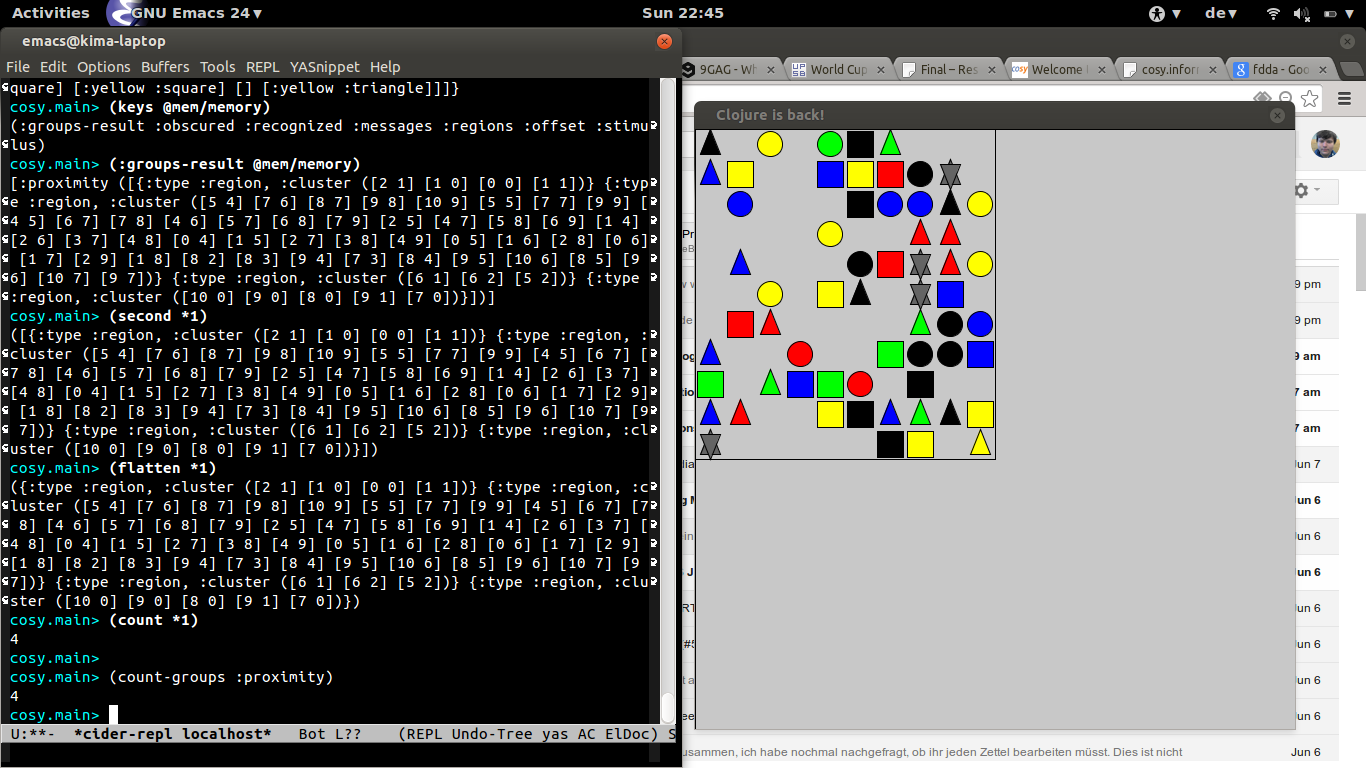
\includegraphics[width=\textwidth]{grouping_example}
     \caption{Recognizing 4 groups of proximity}
     \label{fig:aufbau}
 \end{figure}
\end{frame}
\begin{frame}[label=sec-7]{\#2}
\begin{figure}[hbtp]
     \centering
     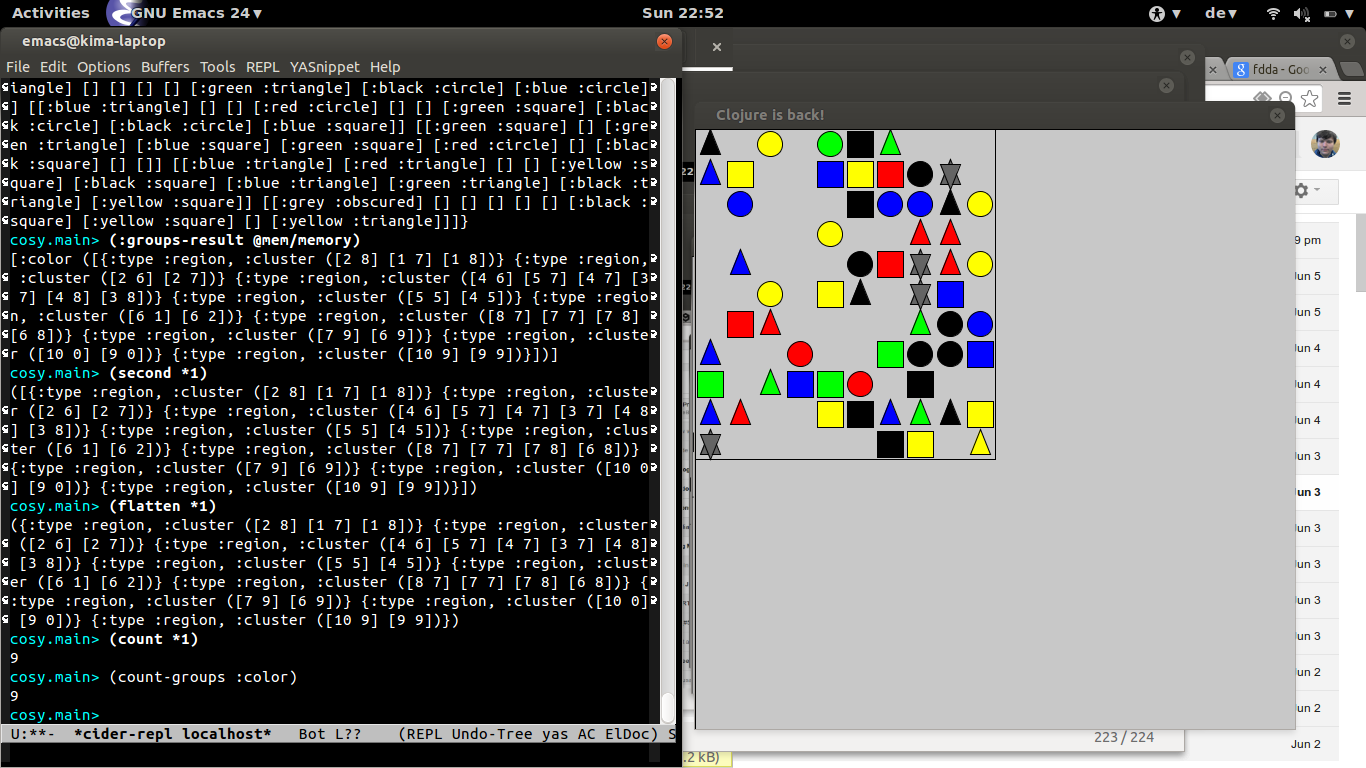
\includegraphics[width=\textwidth]{color_groups_example}
     \caption{Recognizing the groups of color}
     \label{fig:aufbau}
 \end{figure}
\end{frame}
\begin{frame}[label=sec-8]{\#3}
\begin{figure}[hbtp]
     \centering
     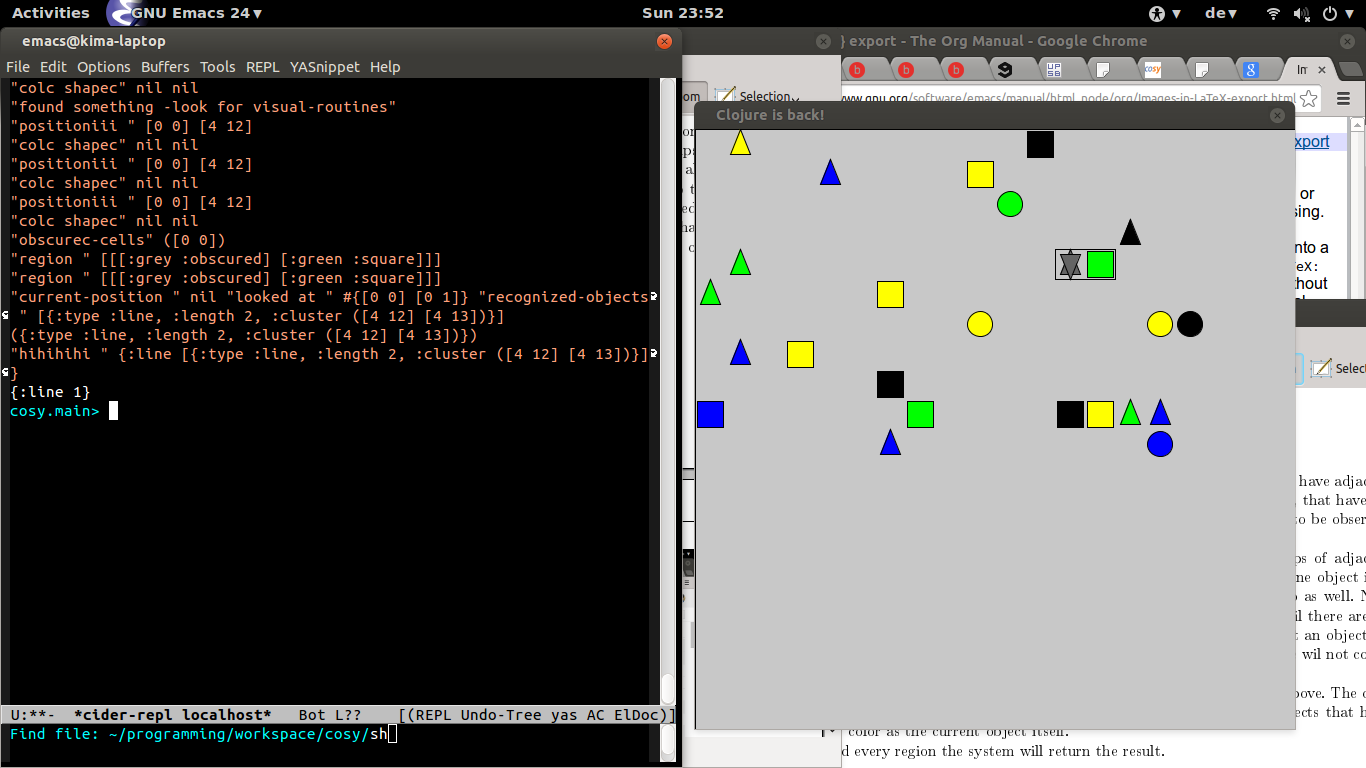
\includegraphics[width=\textwidth]{count_obscured}
     \caption{Recognizing one line-like object}
     \label{fig:aufbau}
 \end{figure}
\end{frame}
\begin{frame}[label=sec-9]{\#4}
\begin{figure}[hbtp]
     \centering
     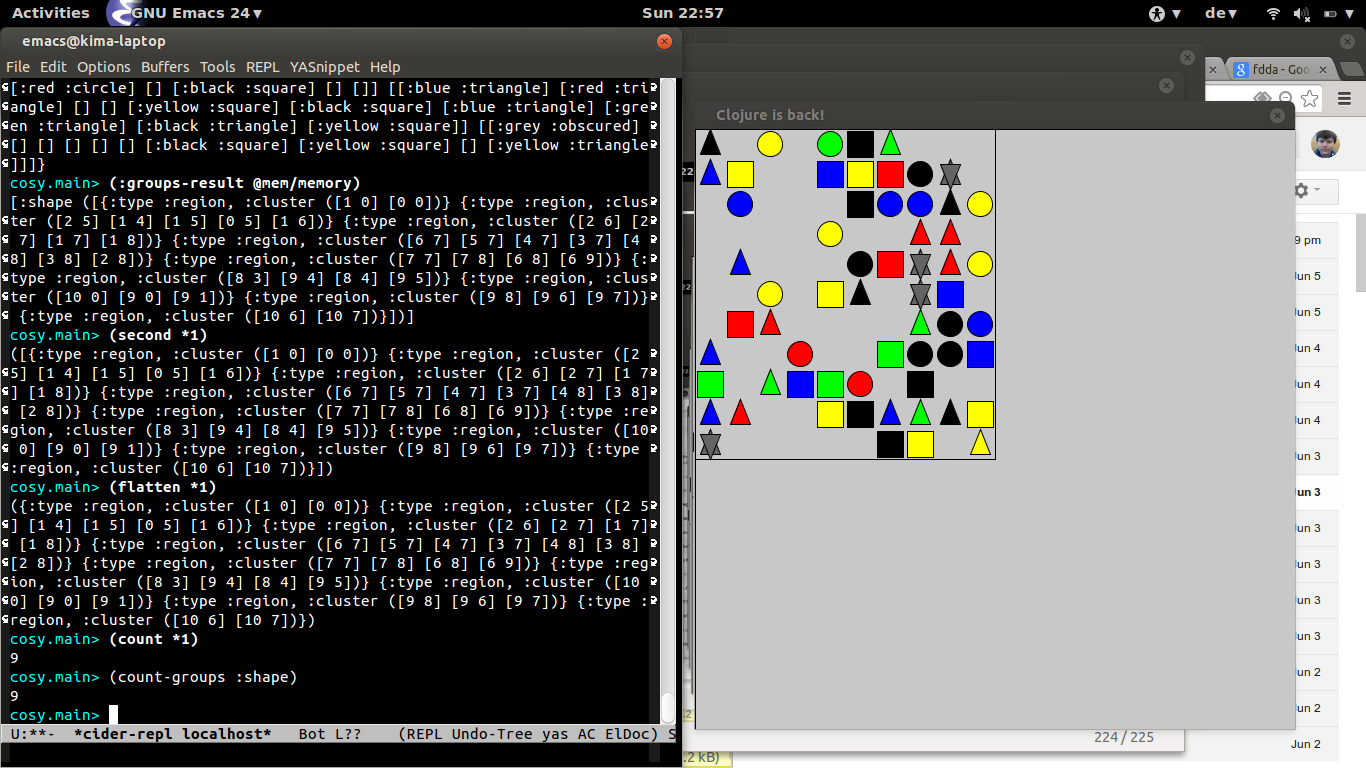
\includegraphics[width= 0.7 \textwidth]{shape_group_example}
     \caption{Recognizing the groups of shape}
     \label{fig:aufbau}
 \end{figure}
\end{frame}

\begin{frame}[label=sec-10]{\#5}
 \begin{figure}[hbtp]
    \centering
    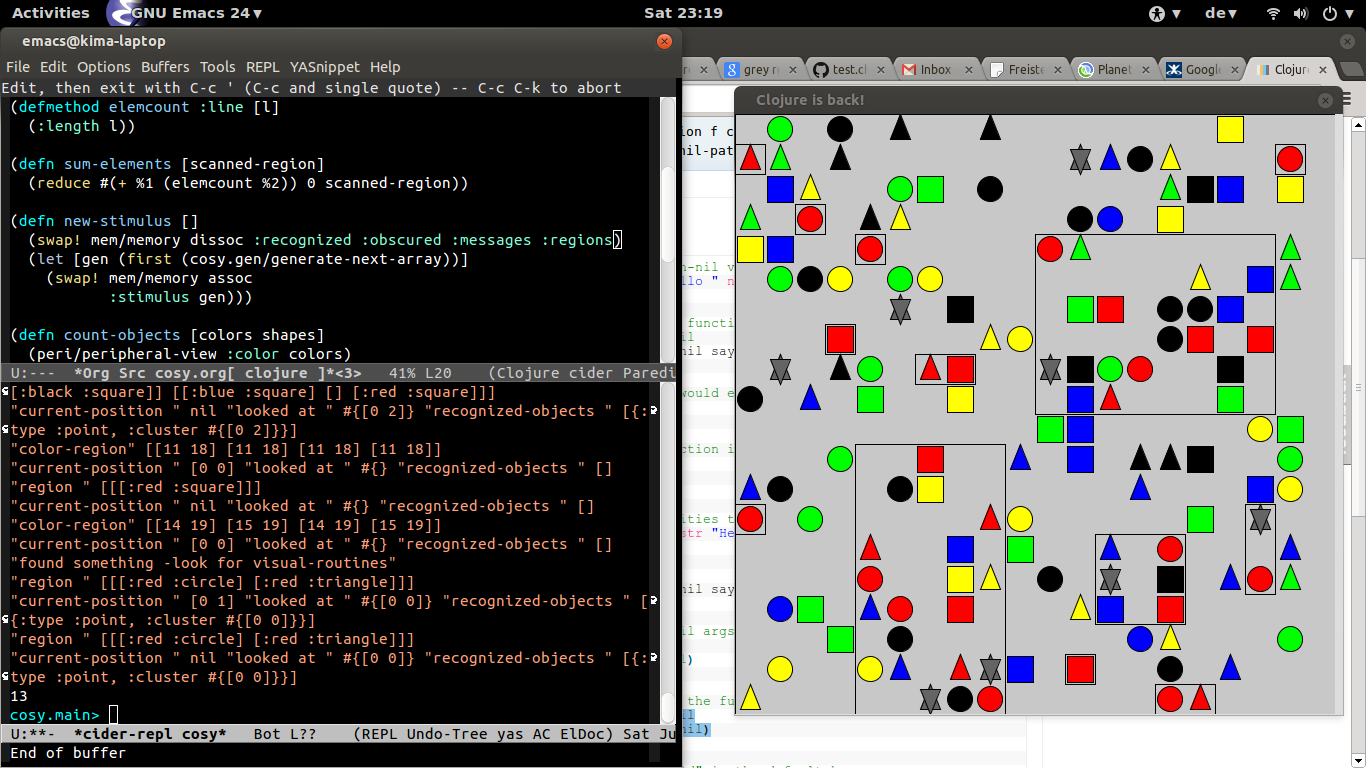
\includegraphics[width= 0.7 \textwidth]{count_red_circles}
    \caption{counting - including obscured objects}
    \label{fig:aufbau}
\end{figure}
\end{frame}
% Emacs 24.3.1 (Org mode 8.2.6)
\end{document}